% !TEX TS-program = pdflatex
% !TEX encoding = UTF-8 Unicode

\documentclass[10pt,twocolumn]{article}

\usepackage{graphicx,listings,fixltx2e,lambda,array,times,fullpage}
\usepackage[usenames,dvipsnames]{xcolor}
\usepackage{color}

\definecolor{lightgray}{rgb}{0.92,0.92,0.92}

\lstset{ 
  language=Python,                % the language of the code
  linewidth=220pt, 
  xleftmargin=8pt,
  basicstyle=\footnotesize\ttfamily, % Standardschrift
  numbers=none,                   % where to put the line-numbers
  numberstyle=\footnotesize,          % the size of the fonts that are used for the line-numbers
  stepnumber=1,                   % the step between two line-numbers. If it's 1, each line 
                                  % will be numbered
  numbersep=5pt,                  % how far the line-numbers are from the code
  showspaces=false,               % show spaces adding particular underscores
  showstringspaces=false,         % underline spaces within strings
  showtabs=false,                 % show tabs within strings adding particular underscores
  frame=single,                   % adds a frame around the code
  tabsize=2,                      % sets default tabsize to 2 spaces
  captionpos=b,                   % sets the caption-position to bottom
  breaklines=true,                % sets automatic line breaking
  breakatwhitespace=false,        % sets if automatic breaks should only happen at whitespace
  title=\lstname,                   % show the filename of files included with \lstinputlisting;
                                  % also try caption instead of title
  numberstyle=\tiny\color{gray},        % line number style
  keywordstyle=\color{blue},          % keyword style
  commentstyle=\color{dkgreen},       % comment style
  backgroundcolor=\color{lightgray}, 
  belowskip=-10pt, 
  aboveskip=6pt, 
}


\begin{document}

\title{Parakeet: A Just-In-Time Parallel Accelerator for Python}
\author{
Alex Rubinsteyn \ \ \ \ Eric Hielscher \ \ \ \ Nathaniel Weinman \ \ \ \
Dennis Shasha \\
{\it Computer Science Department, New York University, New York, NY, 10003} \\
\small{\tt \{alexr,hielscher,nsw233,shasha\} @ cs.nyu.edu}
}
\date{}

% define some useful commands to use in language specification 
\newcommand{\MAP}{\impfnt{map}}
\newcommand{\REDUCE}{\impfnt{reduce}}
\newcommand{\SCAN}{\impfnt{scan}}
\newcommand{\ALLPAIRS}{\impfnt{allpairs}}
\newcommand{\concat}{\ensuremath{+\!\!\!\!+\,}}

\setlength\fboxsep{8pt}
\setlength\fboxrule{0.5pt}

\maketitle

\begin{abstract}
High level productivity languages such as Python or Matlab enable the use of computational resources by non-expert programmers.  However, these languages sacrifice program speed for ease of use, with this trade-off especially stark for modern parallel processors such as multicore CPUs and manycore GPUs.

In this paper, we discuss Parakeet, a library which provides a just-in-time (JIT) parallel accelerator for Python.  Parakeet bridges the gap between the usability of Python and the speed of code written in efficiency languages such as C++ or CUDA.  Parakeet accelerates data-parallel sections of Python that use the standard NumPy scientific computing library.  Parakeet automatically JIT compiles efficient versions of Python functions and manages their execution on both GPUs and multicore CPUs.  We assess Parakeet on a pair of benchmark programs and exhibit significant speedups.  We use these current results as a basis for discussing our plans to augment the Parakeet feature set.
\end{abstract}

\section{Introduction}
\label{Intro}
Computers are indispensable tools to professionals in a wide range of fields, from the natural sciences to the financial industry.  Often, users in these fields either (1) aren't expert programmers; or (2) don't have time to spend on writing and tuning their software for performance.  Thus, these users typically prefer to use productivity languages such as Python or Matlab as opposed to efficiency languages such as C++.  Productivity languages facilitate non-expert programmers by trading off program speed for ease of use \cite{Pre03}.

A common problem, however, is that the performance tradeoff is often very stark -- code written in Python or Matlab~\cite{Moler80} often has much worse performance than code written in C++ or Fortran.  This problem is getting worse, as modern processors (both multicore CPUs as well as manycore GPUs) are all parallel, and current implementations of productivity languages are poorly suited for parallelism.  Thus a common workflow involves rapid prototyping of algorithms in a productivity language, followed by porting the performance-critical sections to an efficiency language so as to achieve tolerable performance.  This second step can be time-consuming, error-prone, and diverts energy from the real focus of these users' work.

% Heart of Parakeet - an interpreter for our high level IL w/ array ops
In this paper, we present Parakeet, a library that provides a JIT parallel accelerator for NumPy, the commonly-used scientific computing library for Python~\cite{Oliphant07}. Parakeet accelerates performance-critical sections of numerical Python programs to be competitive with efficiency language code, obviating the need for the above-mentioned ``prototype, port'' cycle.

The Parakeet library intercepts functions that have been marked with a decorator, and uses high-level operations on NumPy arrays (e.g.~mapping a function over the array's elements) as sources of parallelism. These functions are just-in-time compiled to either x86 machine code using LLVM~\cite{Latt02}, or GPU programs that can be executed on NVIDIA GPUs via the CUDA framework~\cite{NvidCU}. These native versions of the functions are then automatically executed on the appropriate hardware. Parakeet allows complete interoperability with all of the standard Python tools and libraries.

Parakeet currently supports JIT compilation to parallel GPU programs and single-threaded CPU programs.  While Parakeet is a work in progress, our current results clearly demonstrate its promise.  In the near future, Parakeet's CPU support will be extended to make better use of modern multicore processors.  This includes adding support for splitting computations across CPUs and GPUs simultaneously -- keeping all processors in a system busy at once -- and on-the-fly tuning of resource usage.

\section{Overview}
\label{overview}

Parakeet is an accelerator library for numerical Python algorithms written using the NumPy array extensions~\cite{Oliphant07}. Parakeet does not replace the standard Python runtime but rather selectively augments it. To run a function within Parakeet a user must wrap it with the decorator \lstinline{@PAR}. For example, consider the following NumPy code for computing the entropy of a discrete probability distribution. 
\begin{lstlisting}
  @PAR
  def entropy(p):
    return -numpy.sum(p * numpy.log2(p))
\end{lstlisting}
If the decorator \lstinline{@PAR} were removed, then \lstinline{entropy} will run as ordinary Python code. Since NumPy's \lstinline{log2} and array multiplication operators are statically compiled they will allocate array result even if it will be immediately consumed. By contrast, Parakeet specializes the function \lstinline{entropy} for any distinct input type, optimizes the body into a singled fused reduction (avoiding unnecessary allocation) and finally executes it as parallel native code.


%We have implemented two backends for Parakeet: a manycore GPU backend on top of CUDA and a less mature multicore backend using LLVM. Both of these backends rely on the presence of 
%data parallel 


Parakeet is not meant as a general-purpose accelerator for all Python programs.  Rather, it is designed to execute array-oriented numerical algorithms such as those found in machine learning, financial computing, and scientific simulation. In particular, the sections of code that Parakeet accelerates must obey the following constraints:

\begin{itemize}
 \item Due to the difficulty of implementing efficient non-uniform data structures on the GPU, we require all values within Parakeet to be either scalars or NumPy arrays. No dictionaries, sets, or user-defined objects are allowed. 
 \item To compile Python into native code we must assign types to each expression in a function. We are still able to implement some of Python's polymorphism by specializing different typed versions of a function for each distinct set of argument types. However, expressions whose types depend on dynamic values (such as \lstinline{43 if bool_val else "sausage"}) are disallowed.
 \item Only functions which don't modify global state or perform I/O can be executed in parallel. Local mutabable variables are however always allowed. 
\end{itemize}

These restrictions would be onerous if applied to an entire program, but it's important to remember that Parakeet only sees the computational core of an algorithm. All other code is executed as usual by the Python interpreter. Furthermore, the style of programming required for Parakeet matches closely to the idiomatic conventions of array programming. In practice, if an algorithm makes heavy use of NumPy operators for its computations then it will run under Parakeet with only minor modifications. 

Though Parakeet supports the use of loops, it does not attempt to in any way parallelize them. Parallelism is instead achieved by relaxing the iteration order of the following higher-order array operators. 

\begin{itemize}
\item $\MAP(\textit{f}, \; \textit{X}_1,  ... ,  \textit{X}_n, \; \textit{fixed}\textrm{=[]}, \; \textit{axis}\textrm{=None})$ \\
      Apply the function \textit{f} to each element of the array arguments. By default, \textit{f} is passed each scalar element of the array arguments. The axis keyword
      can be used to specify a different iteration pattern (such as applying \textit{f} to all columns). 
      The \textit{fixed} keyword is a list of values which precede the array elements as arguments to \textit{f} (simulating partial function application). 
       
\item $\ALLPAIRS(\textit{f}, \; \textit{X}_1,  \; \textit{X}_2, \; \textit{fixed}\textrm{=[]}, \; \textit{axis}\textrm{=} 0)$ 
\item $\REDUCE(\textit{f}, \; \textit{X}_1,  ... ,  \textit{X}_n, \; \textit{fixed}\textrm{=[]}, \; \textit{axis}\textrm{=None}, \; \textit{init}\textrm{=None})$
\item $\SCAN(\textit{f}, \; \textit{X}_1,  ... ,  \textit{X}_n, \; \textit{fixed}\textrm{=[]}, \; \textit{axis}\textrm{=None}, \; \textit{init}\textrm{=None})$
\end{itemize}

If the axis argument is omitted then the function is applied to every scalar element of the arrays. 
Examples: 
map(sqrt, array([1,4,9]))  \# evaluates to array([1,2,3])
map(sum, array([[1,2,3],[4,5,6]), axis=1) \# evaluates to array([5, 7, 9])
allpairs(lambda x,y: sqrt((x-y)*(x-y)), X, Y) \# distance between all pairs of rows
reduce(np.add, array([1,2,3])) \# evalutes to 6 

scan(np.add, array([1,2,3])) \# evaluates to array([1,3,6])



These "data parallel" operators par basic units of parallelism in Parakeet are the following data parallel operators. 
Array operations encode rich information about their access patterns that we can exploit to translate them into efficient parallel programs \cite{Ju94}

%Might be useful: 
% .


\subsection{Code Example}
Let's make things more concrete with a code example.  Figure \ref{MinIdx} shows two functions that form part of the K-Means clustering benchmark we use to evaluate Parakeet in Section \ref{Evaluation}.  The \texttt{minidx} function takes two inputs: a matrix \texttt{C} of vectors, and another vector \texttt{x}.  It computes the index of the vector in \texttt{C} whose distance from \texttt{x} is the smallest.

The program execution pipeline for NumPy code by Parakeet (shown in Figure \ref{fig:overview}) begins in the standard Python interpreter. At program start time, a subset of the program's functions (annotated manually by the programmer with a function decorator) are registered with Parakeet as potentially accelerable. The body of a registered function is then translated into an untyped intermediate representation using the Parakeet front end interface and the Python's introspection facilities.

\begin{figure}[h!]
\begin{lstlisting}[language=Python,frame=single]
def sqr_dist(x,y):
  return sum((x-y) * (x-y))

@PAR
def minidx(C,x):
  sqr_dists = map(sqr_dist,C,fixed=[x])
  return argmin(sqr_dists)
\end{lstlisting}
\caption{Minimum Distance Example}
\label{MinIdx}
\end{figure}

When a call is made to a function which has been registered with Parakeet, the untyped function is specialized by propagating type information from the arguments to all values in the body.  Type specialization translates the function into a typed intermediate language. Further standard optimizations are performed at this stage, the most impactful of which is \emph{array operator fusion}, wherein array operations are combined according to rewriting rules. This fusion step can be extremely beneficial to the final program's performance, especially when executed on the GPU, as it can drastically increase computational density and eliminate many wasteful array temporaries.

Execution of the optimized typed IL is initiated by Parakeet's interpreter, which is then responsible for deciding which operations to JIT compile to native code for the CPU or GPU. When the interpreter encounters an array operator it employs a simple cost-based heuristic (which considers nested array operators, data sizes, and memory transfer costs) to decide where to execute it (for more details see Section \ref{costmodel}). Parakeet's interpreter invests great effort into analyzing both the program and information about the data to make dynamic execution decisions. The cost of these analyses are mitigated by the tremendous computational density of the intermediate language's array operators.

If an array operator's computation is deemed a good candidate for native hardware execution, Parakeet flattens all nested array computations within that operator into sequential loops.  This payload is then inlined into a program skeleton that implements that operator.  For example, in the case of a \textbf{map} operation, Parakeet provides skeletal algorithms that implement the pattern of applying the same function to each element of an array on the CPU as well as on the GPU.  The flattened payload function argument is inlined into this skeleton, and a complete program is synthesized and JIT compiled.

To execute the native code, Parakeet first copies any of its inputs that aren't already present in the memory of the target hardware to their necessary place.  Parakeet manually manages the memory of the system, for example treating the GPU's memory as a cache of data whose canonical values are the CPU's RAM. The program is then executed, with memory reclaimed via garbage collection.

\begin{figure*}[t!bh]
\begin{center}
\leavevmode
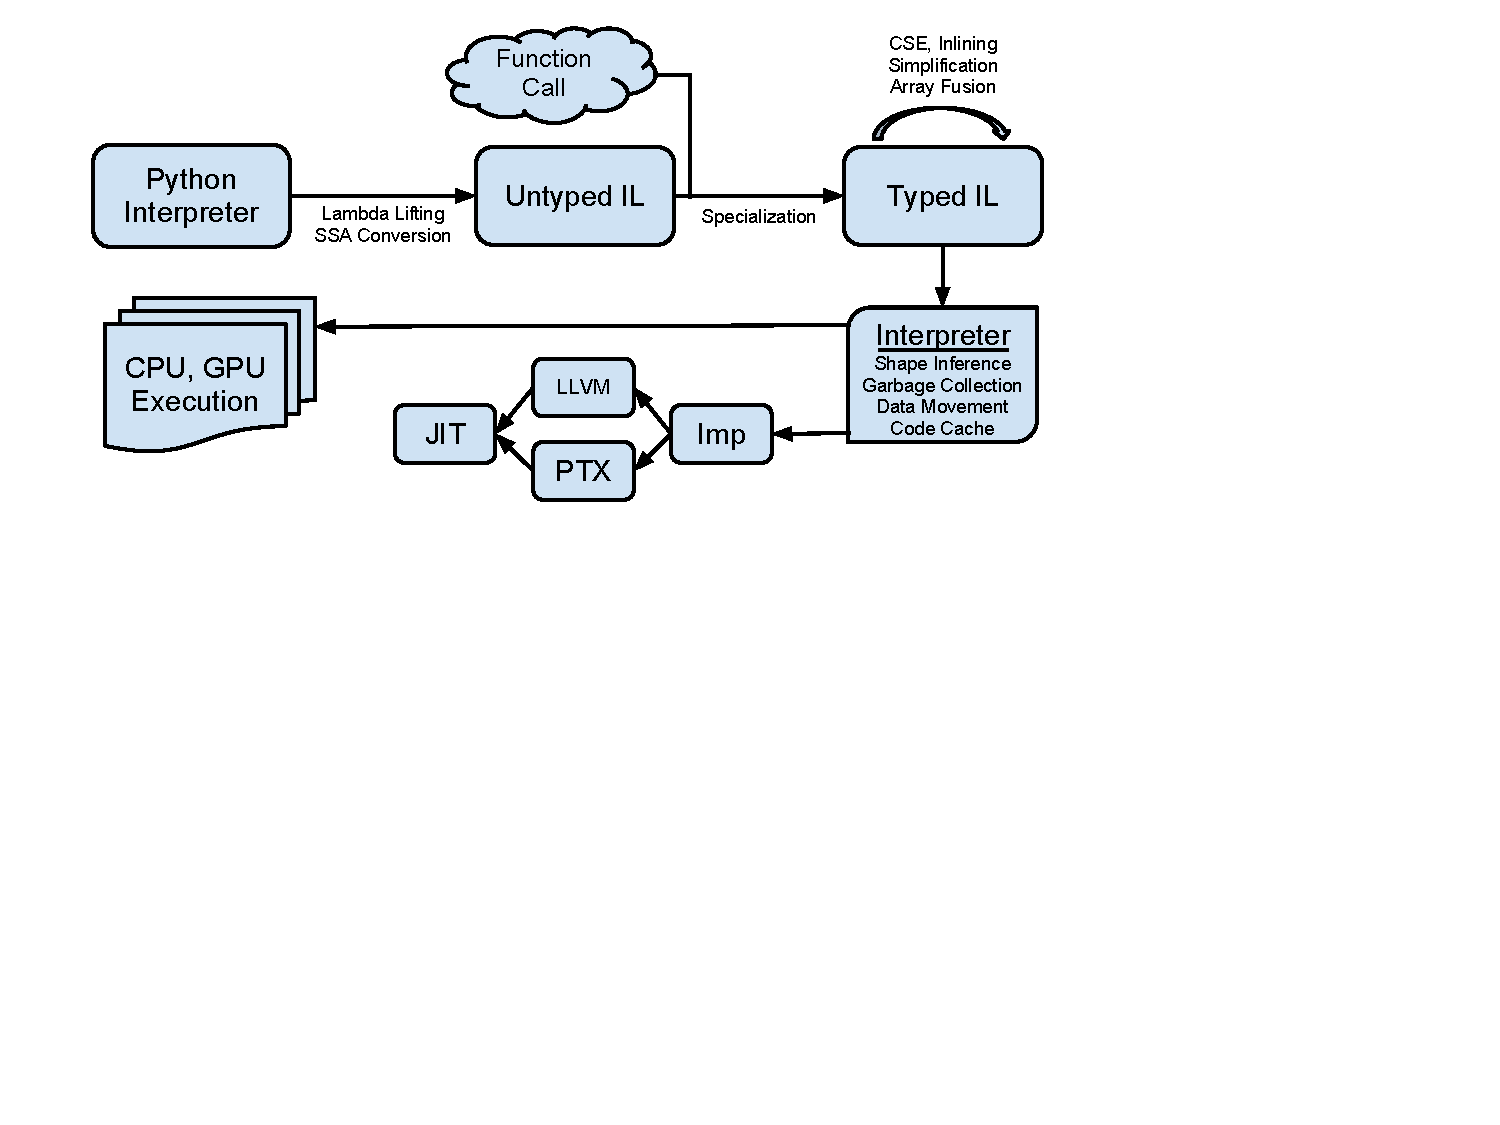
\includegraphics[scale=0.6, trim=0pt 310pt 140pt 80pt]{ParakeetNumPyOverview.pdf}
\end{center}
\caption{Parakeet Pipeline}
\label{fig:overview}
\end{figure*}

\section{Parakeet Pipeline}
\label{Pipeline}
Now we turn to the problem of compiling an array language program into an efficient GPU program. At first glance, there seems to be a significant mismatch between the highly dynamic expressiveness of an array language like Q and the limitations imposed by GPU hardware discussed in Section \ref{GPULimitations}. Indeed, the Parakeet intermediate language must serve as a compromise between two competing tensions. In order to translate array programs into efficient GPU code it is necessary for the compiler to eliminate as much abstraction as possible. On the other hand, we must be careful not to make our program representation overly concrete with regard to evaluation order (which would eliminate opportunities for parallelism provided by the array operators). 
\textit{In deference to the above-mentioned GPU hardware restrictions, any program which is compiled to run on the GPU cannot have any of the following:}


\subsection{Lambda Lifting and SSA Conversion}
After a function call has been intercepted by the Parakeet runtime, Parakeet performs a syntax-directed translation from a language-specific abstract syntax tree (AST) into Parakeet's IL. Since type information is not yet available to specialize user functions, the functions must be translated into an untyped
form. 

\subsection{Untyped Optimizations}
Parakeet performs optimizations both before and after type specialization. We subject the untyped representation to inlining, common subexpression elimination and simplification (which consists of simultaneous constant propagation and dead code elimination). This step occurs once for each function, upon its first interception by Parakeet. It is preferable to eliminate as much code as possible at this early stage since an untyped function body serves as a template for a potentially large number of future specializations. The only optimizations we do not perform on the untyped representation are array fusion rewrites, since these rely on type annotations to ensure correctness.

\subsection{Specialization}
Specialization transform user programs from the untyped intermediate language into its typed variety. The purpose of this transformation is to eliminate polymorphism, to make manifest all implicit behavior (such as coercion and scalar promotion), and to assign simple unboxed types to all data used within a function body. Beyond the fact that the GPU requires its programs to be statically typed, these goals are also essential for the efficient execution of user code on the GPU. Thus, the specializer generates a different specialized version of a function for each distinct call string, with all of the function's variables receiving the appropriate types.

We take inspiration from \cite{Bol09} and allow functions to both accept and return multiple values. This feature simplifies the specification of certain optimizations and naturally models the simultaneous creation of multiple values on the GPU. 

\textit{This representation of function values resembles defunctionalization combined with specialization of \textit{apply} functions \cite{Tolmach98}. }

\subsection{Array Operator Fusion}
In addition to standard compiler optimizations (such as constant folding, function inlining, and common sub-expression elimination), we employ fusion rules~\cite{Jones01} to combine array operators. Fusion enables us to minimize kernel launches, boost the computational density of generated kernels, and avoid the generation of unnecessary array temporaries.

We present the fusion rules used by Parakeet in simplified form, such that array operators only consume and produce a single value. Our rewrite engine generalizes these rules to accept functions of arbitrary input and output arities.
\\[5pt]
\begin{tabular}{|m{0.001cm} m{0.05cm} p{6.5cm} p{0.05cm} |}
  \hline 
  & &  & \\
  & \multicolumn{2}{l}{\large{Map Fusion} }  &  \\[2.5pt]
  & & $\MAP(g, \MAP(f, x)) \leadsto \MAP(g \circ f, x)$ & \\
  & & & \\
  & \multicolumn{2}{l}{\large{Reduce-Map Fusion} }  & \\[2.5pt]
  & & $\REDUCE(g, \MAP(f, x)) \leadsto \REDUCE(g \circ f, x)$ & \\
  & & & \\
  \hline
\end{tabular}\\[4pt]

These transformations are safe if the following conditions hold:
\begin{enumerate}
\item All the functions involved are referentially transparent.

\item Every output of the predecessor function ($f$) is used by the successor
($g$).

\item The outputs of the predecessor are used \textit{only} by the successor.
\end{enumerate}

The last two conditions restrict our optimizer from rewriting anything but linear chains of produced/consumed temporaries. A large body of previous work~\cite{Ald01} has demonstrated both the existence of richer fusion rules and cost-directed strategies for applying those rules in more general scenarios. Still, despite the simplicity of our approach, we have observed that many wasteful temporaries in idiomatic array code are removed by using only the above rules.



\section{The Parakeet Runtime}
\label{runtime}

Once a function has been type specialized and fully optimized, it is handed off to the Parakeet runtime for intelligent execution. The heart of the runtime is a heavy-weight interpreter whose primary responsibility is to initiate GPU kernel synthesis and execution. The interpreter uses program analyses and performance heuristics in order to dynamically make decisions such as: 
\begin{enumerate}
\item what portion of a user's program ought to run on the GPU 
\item which level of nested parallelism ought to expressed as a GPU kernel
\item in which GPU memory space should a particular array reside 
\item when should data be moved onto or off the GPU
\end{enumerate} 

\subsection{Cost Model}
\label{costmodel}

When the Parakeet interpreter encounters an array operator, it uses a simple cost model to decide what is the best place to execute the operator.  The cost model employs a recursive function that estimates the relative cost of executing that operator on the CPU versus the GPU.  This function is not meant to measure the precise expected run time of the operator; rather, the goal is to make the correct decision when the use of one or the other processor should result in much higher performance.  We use the clock frequency of each processor to roughly estimate the cost of a single operation.  For each array operator, we multiply the estimated cost of a single execution of the operator's function argument by some fixed function of the input size.  For a \textbf{map} operation, for example, we multiply the estimated cost of performing the sequentialized version of the mapped function by the number of input elements. In addition, we estimated the time needed to transfer data to and from the GPU as a function of data size and add this cost to the total if the data is not already present in the respective processor's memory.

In the case of nested array operators -- e.g.~a \textbf{map} whose payload function is itself a \textbf{reduce} the interpreter needs to choose which operator, if any, will form the parallelization point for a GPU kernel while sequentializing all nested operators within that kernel.  The possible choices include:

\begin{enumerate}
\item Running the \textbf{map} as a GPU kernel, with an embedded sequential \texttt{for} loop that implements the \textbf{reduce}.
\item Running the \textbf{map} as a \texttt{for} loop in the Parakeet interpreter, with each iteration of the loop calling a GPU kernel that implements the \textbf{reduce}.
\item Running everything in the Parakeet interpreter as two nested \texttt{for} loops.
\end{enumerate}

In cases (1) and (3), the operator is executed entirely on a single processor.  In case (2), however, the \textbf{map} runs as a loop on the CPU, generating each element of the resulting vector with a separate GPU program invocation.  In this case, the interpreter creates an interpreter array object on the CPU whose elements are references to the values generated on the GPU.  The final linear CPU array is only constructed lazily as needed or when the GPU garbage collector needs the space.  At that point, a linear CPU array is allocated and filled in with the computed values.  This is precisely what happens in our implementation of K-Means clustering discussed in Section \ref{results-k-means}.

\subsection{Shape Inference}
\label{shapeinference}
Accurate prediction of array shapes is necessary both for the allocation of intermediate values on the GPU as well as for the above cost model determining placement of computations. We employ a simple abstract interpreter which propagates shape information through a function using the obvious shape semantics for each operator. For example, a $\REDUCE$ operation collapses the outermost dimension of its argument whereas a $\MAP$ preserves a shape's outermost dimension.

\subsection{Data Movement and Garbage Collection} 
Arrays are moved to the GPU whenever they are used as the argument to some GPU computation. The specific GPU memory space into which an array is loaded depends on both the other data already on the GPU and the individual characteristics of the computation in which that array is being used.
Unlike some systems similar to Parakeet \cite{Chaf11}, we do not by default preallocate the entirety of the GPU's memory.  Rather, Parakeet has a runtime flag that can enable such preallocation for better performance in dedicated compute server environments.  This is because we expect a typical use case to be in a desktop environment, where the GPU serves a double function of graphics processing and array operator acceleration and we don't want steal all of the GPU's resources.

Tracking and collection of unused memory is achieved by counting array references. Parakeet does not immediately free an array whose reference count drops to zero but rather maintains a cache of free data blocks which can be cheaply reused. Such caching of free pointers can be advantageous when a computation repeatedly allocate arrays of the same size. 

\subsection{Data Layout}
\label{datalayout}

Parakeet is able to leverage dynamic information in various ways to optimize both the implementation and the execution of the GPU programs it executes.  One important such optimization is automated data layout.  On GPUs, poor memory access patterns can result in orders of magnitude lower performance.  In particular, neighboring threads in an executing GPU kernel should access adjacent memory words in order to get maximum performance.  Use of column major data layouts as a performance optimization is well known in the CPU high performance computing world.  Parakeet's data layout is row major by default.  However, when a \textbf{map} computation is performed over a two-dimensional structure, a row major layout would result in the worst possible memory access pattern for the GPU kernel as its threads would concurrently access memory at some large stride.  Thus in this case, Parakeet specializes the function in question to create a transposed column-major version of the data input.  This column-major version is strictly an intermediate within the Parakeet runtime.  We have found this optimization to be extremely beneficial to performance, and it contributes immensely to the good performance Parakeet delivers on the K-Means clustering benchmark discussed in Section \ref{results-k-means}.

\section{GPU Back End}
Several systems similar to Parakeet \cite{Cata11,Chaf11} generate GPU programs by emitting CUDA code which is then compiled by NVIDIA's CUDA nvcc toolchain. Parakeet on the other hand, targets PTX, which is NVIDIA's GPU pseudoassembly language. Parakeet's PTX code is dynamically compiled by the NVIDIA graphics driver before being executed.  Parakeet caches compiled binaries so that when a particular array operator is run multiple times on the GPU with similar arguments it needn't incur the code generation and JIT compilation costs more than once.

We prefer compiling PTX instead of CUDA since this enables us to generate binaries more quickly, achieving a fully dynamic compiler without any noticeable stalls. The NVIDIA CUDA compiler is a wrapper around the GCC C++ compiler, and CUDA supports all of C++ in the host code and a large subset (including C++ templates) in the GPU code.  Thus, the compile times for even simple kernels can be on the order of 5--10 seconds.  There are, of course, advantages to using the NVIDIA compiler. The main ones are that we would be able to take advantage of all of the NVIDIA and GCC compiler optimizations and that it would simplify our implementation effort.  

\subsection{Imp}
\label{Imp}
As mentioned above, we implement the higher-order array operators as skeletons of code with splice points where their payload functions get inlined.  Rather than implement these skeletons directly in CUDA or PTX, Parakeet utilizes an embedded DSL called Imp, which operates at a semantic level similar to CUDA. Imp is intentionally a very simple language, since its purpose is to facilitate quick compilation from the typed IL to PTX. 

Space requirements of a function call (all outputs and local arrays it must allocate) can be determined as a function of input sizes. This is necessary as GPU computations have access only to memory which is allocated before their launch and cannot ``dynamically'' allocate more memory.

Imp kernels are ``shapely'' by construction, meaning they specify their memory requirements as deterministic functions of input size. This obviates the need for ad-hoc allocation logic (the bulk of most CUDA host code in practice) or for auxiliary size inference on higher level code. If a function can be translated to Imp then we can always determine its memory requirements.

\section{Evaluation}
\label{Evaluation}

We evaluated Parakeet on two benchmarks: Black-Scholes option pricing, and K-Means Clustering.  We compare Parakeet against both hand-tuned CPU and GPU implementations.  Due to space constraints, and since at the time of writing our CPU backend only supports single-threaded execution, we only present Parakeet results for its GPU backend.  For Black-Scholes, the CPU reference implementation is taken from the PARSEC \cite{Bien08} benchmark suite, and the GPU implementation is taken from the CUDA SDK \cite{NvidSD}.  For K-Means Clustering both the CPU and GPU benchmark versions come from the Rodinia benchmark suite~\cite{Che09}.

We ran all of our benchmarks on a machine running 64-bit Linux with an Intel Core i7 3.2GHz 960 4-core CPU  and 16GB of RAM.  The GPU used in our system was an NVIDIA Tesla C1060 with 240 vector lanes, a clock speed of 1.296 GHz, and 4GB of memory.

\subsection{Black-Scholes}
\label{results-bs}

Black-Scholes option pricing \cite{Blac73} is the standard algorithm used for data parallel benchmarking.  We compare Parakeet against the multithreaded OpenMP CPU implementation from the PARSEC \cite{Bien08} benchmark suite with both 1 and 8 threads and the CUDA version in the NVIDIA CUDA SDK \cite{NvidSD}.  We modified the benchmarks to all use the input data from the PARSEC implementation so as to have a direct comparison of the computation alone.  We also modified the CUDA version to calculate only one of the call or put price per option so as to match the behavior in PARSEC.

\begin{figure}[h!]
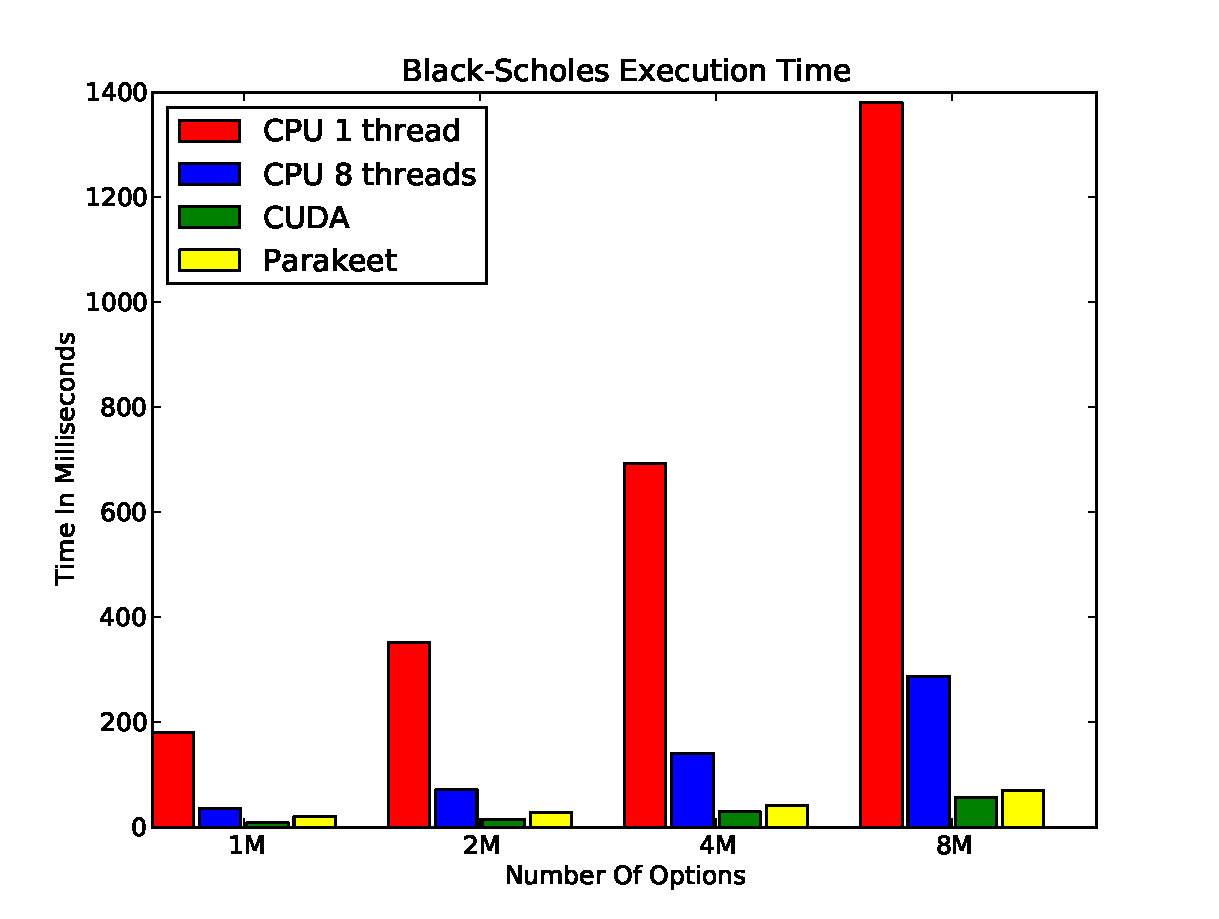
\includegraphics[scale=0.4]{BSWCPU.pdf}
\caption{Black Scholes Total Times}
\label{BSCPU}
\end{figure}

In Figure \ref{BSCPU}, we see the total run times on the various systems. These times include the time it takes to transfer data to and from the GPU in the GPU benchmarks.  As expected, Black Scholes performs very well on the GPU as compared with the CPU.  We see that Parakeet performs very similarly to the hand-written CUDA version, with overheads decreasing as a percentage of the runtime as the data sizes grow since most of them are fixed costs related to dynamic compilation.

\subsection{K-Means Clustering}
\label{results-k-means}

\begin{figure}
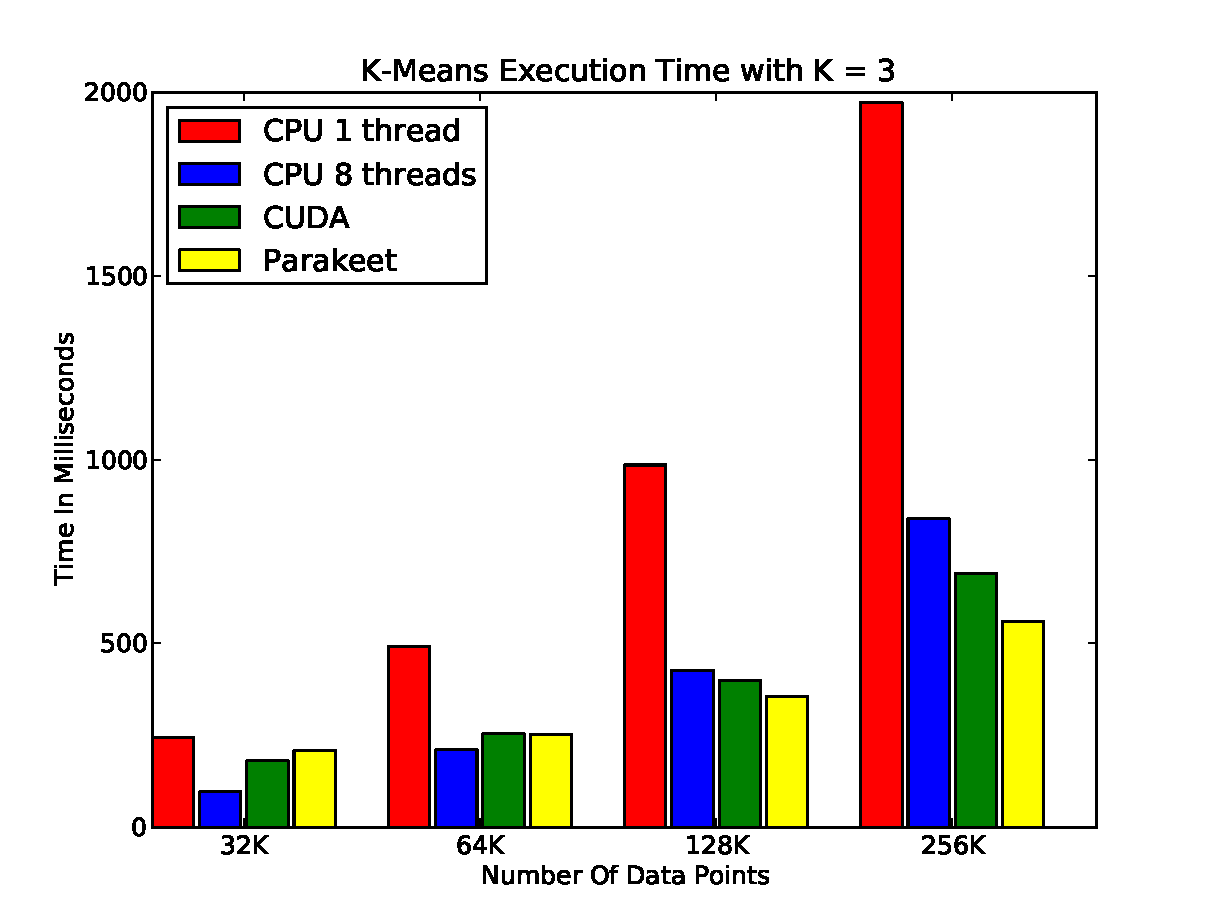
\includegraphics[scale=0.4]{KMCPUK3.pdf}
\caption{K-Means Total Times with 30 Features, K = 3}
\label{KMCPU3}
\end{figure}

We also tested Parakeet on K-Means clustering, a commonly used unsupervised learning algorithm.  We chose K-Means since it includes both sequential loops and nested array operators, and thus illustrates Parakeet's support for both.

In Figure \ref{KMCPU3}, we see the total run times of K-Means for the CPU and GPU versions with K = 3 clusters and 30 features on varying numbers of data points.  Here, the distinction between the GPU and the CPU is far less stark.  In fact, for up to 64K data points the 8-thread CPU version outperforms the GPU.  Further, we see that on all but the smallest input size, Parakeet actually performs better than both the CPU and GPU versions.

The reason Parakeet is able to perform so well with respect to the CUDA version is due to the difference in how the two versions execute the code that computes the new average centroid for the new clusters in each iteration.  The CUDA version brings the GPU-computed assignment vectors back to the CPU in order to perform this reduction, as it involves many unaligned memory accesses and so has the potential to perform poorly on the GPU.  Parakeet executes code to perform this function on the GPU instead, prefering to avoid the data transfer penalty.  For such a small number of clusters, the Parakeet method ends up performing far better.  However, for larger numbers of clusters (roughly 30 and above), the fixed overhead of launching an individual kernel to average each cluster's points overwhelms the performance advantage the GPU gives and Parakeet ends up performing worse than the CUDA version.  While we don't take advantage of it yet, this illustrates the potential for using dynamic information to get the best of both worlds.  In the future, in the case of a small number of clusters, Parakeet could execute the averaging code on the GPU, while for larger numbers, it could use a CPU implementation.

\begin{figure}
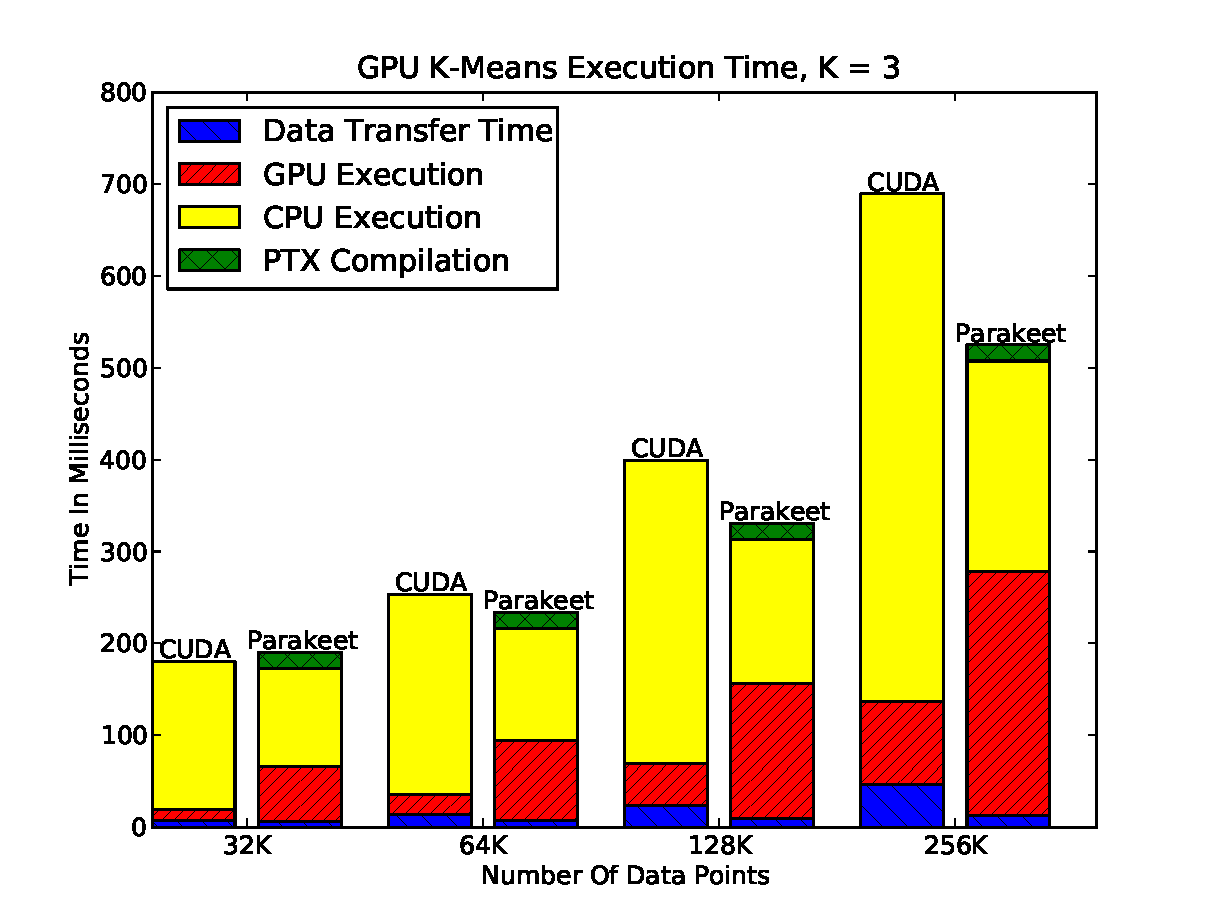
\includegraphics[scale=0.4]{KMGPU.pdf}
\caption{K-Means GPU Times with 30 Features, K = 3}
\label{KMGPU}
\end{figure}

The PTX compilation time is rather significant for this benchmark -- ranging from 33\% of the total runtime for the 1 million option case to roughly 10\% in the 8 million option case.  This cost can't be helped, but it is important to note that it as well as the initialization costs are only paid once per function since Parakeet caches the compiled version of the function.  Thus, in the case of workloads where a single function is repeatedly called, this costs will be insignificant.

In Figure \ref{KMGPU}, we see a breakdown of the run times for CUDA and Parakeet.  Both Parakeet and the CUDA version use the CPU to perform a significant amount of the computation.  The CUDA version uses the CPU to compute the averages of the new clusters in each iteration, while Parakeet spends a lot of time in its interpreter launching many GPU kernels and performing garbage collection of GPU memory.  In addition, we break down the runtime by reported Parakeet's overhead separately.  This overhead includes initialization costs related to registering functions with the Parakeet runtime; time spent in the Parakeet IL interpreter; and the cost of running the JIT compiler on the generated code.  As can be seen, this overhead is small compared with the overall runtime of the benchmark.

\section{Related Work}
\label{RelatedWork}
There have been several projects that use just-in-time compilation to accelerate Python programs on CPUs, but to our knowledge none have generated parallel code.  The PyPy project is an alternative implementation of Python that includes a JIT compiler and boasts an average 5.3X speedup across 20 benchmarks~\cite{Rigo06}. Psyco was a previous Python JIT compiler that boasted decent speedups~\cite{Rigo04}.

The use of graphics hardware for non-graphical computation has a long history~\cite{Leng90}, though convenient frameworks for general purpose GPU programming have only recently emerged. The Brook language extended C with ``kernels'' and ``streams'', exposing a programming model similar to what is now found in CUDA and OpenCL~\cite{Buck04}.  Microsoft's Accelerator~\cite{Tard06} was the first project to use high level (collection-oriented) language constructs as a basis for GPU execution. Accelerator's programming model does not support function abstractions (only expression trees) and its only underlying parallelism construct is limited to the production of $\MAP$-like kernels.

Nikola~\cite{Main10} and Accelerate~\cite{Chak11} are two first-order array-oriented languages embedded within Haskell. Nikola provides a convenient syntax for expressing single-kernel computations, but requires the programmer to manually coordinate computations which require multiple kernel launches and its loop-based parallelization scheme seems ill-fitted to complex array operations.  Unlike Nikola, Accelerate does allow the expression of computations which span multiple kernel launches. Accelerate also has a much richer set of array operators (including the higher-order trio $\MAP$, $\REDUCE$, $\SCAN$). Accelerate, however, does not seem to support closures or the nesting of array operators.

Copperhead parallelizes a statically typed purely functional array subset of Python through the dynamic compilation/execution of CUDA kernels~\cite{Cata11}. Copperhead supports nested array computations, and has a notion of scheduling computation on both GPU and CPU backends (although only a GPU backend has been implemented). In addition to sequentializing nested array operators within CUDA kernels (as done in Parakeet), Copperhead can also share the work of a nested computation between all the threads in CUDA block. Copperhead does not utilize any dynamic information (such as size) when making these scheduling decisions and thus must rely on user annotations. Copperhead's compiler generates kernels through parameterization of operator-specific C++ template classes. By using C++ as their backend target, Copperhead has been able to easily integrate the Thrust ~\cite{Hobe10} GPGPU library and to offload the bulk of their code optimizations onto a C++ compiler.  However, this results in Copperhead's compile times being the longest of any project mentioned here (orders of magnitude longer than the compiler overhead of Parakeet).

\section{Conclusion}
\label{Conclusion}
Parakeet allows the programmer to write Python code using a widely-used numerical computing library while achieving good performance on modern parallel hardware. Parakeet automatically synthesizes and executes efficient native binaries from Python code. Parakeet is a usable system in which complex programs can be written and executed efficiently.  On two benchmark programs, Parakeet delivers performance very competitive with even hand-tuned GPU implementations.  Parakeet code can coexist with standard Python code, allowing full interoperability with all of Python's tools and libraries.

In the near future, we plan to add support for the generation of multithreaded CPU programs to our CPU backend.  In addition, we plan to increase efficiency by iteratively tuning components of hierarchical algorithms, splitting computation simultaneously across all processors in a system, and doing more to overlap computation with data transfers.


{\small
\bibliographystyle{acm}
\bibliography{../Parallelism}{}
}
\end{document}
